\documentclass[11pt,a4paper]{article}
\usepackage[utf8]{inputenc}
\usepackage[T1]{fontenc}
\usepackage[brazilian]{babel}
\usepackage{geometry}
\geometry{margin=2.3cm}
\usepackage{graphicx}
\usepackage{booktabs}
\usepackage{longtable}
\usepackage{array}
\usepackage{float}
\usepackage{xcolor}
\usepackage{amsmath}
\usepackage{enumitem}
\usepackage{caption}
\usepackage{hyperref}
\hypersetup{colorlinks=true, linkcolor=blue!50!black, urlcolor=blue!50!black}
\captionsetup{font=small, labelfont=bf}
\setlist{itemsep=2pt, topsep=4pt}
\graphicspath{{figs/}{../relatorio_ocsvm_cnn1d_mensal/figs/}}
\newcommand{\tg}[1]{\texttt{\detokenize{#1}}}

\title{De onde vêm os falsos positivos da detecção de trips da TC-33003A:\\
causas, hipóteses testadas para eliminá-los e o compromisso que resta\\
\large OCSVM de produção e CNN-1D mensal, 01/2025 a 04/2026 -- Cabiúnas}
\author{Equipe de Modelagem}
\date{19 de outubro de 2026}

\begin{document}
\maketitle

\begin{abstract}
A pipeline de detecção de precursores de trip da turbina TC-33003A pega os 8 trips do histórico, mas emite cerca de
3 alertas por mês de operação que não são seguidos de trip nem de parada: os falsos positivos (FP). Este relatório
procura explicar esses FP: 36 da OCSVM de produção e 45 do CNN-1D com retreino mensal, desde 01/2025. Ele junta
três frentes. (i) A \textbf{composição} dos episódios: quase todo episódio, trip ou FP, nasce do mesmo par de alarmes
recorrentes de processo mais um modelo aceso, quase sempre a vibração. (ii) As \textbf{hipóteses testadas} para
separar trip de FP: tags e temporização do canal de alarmes, debounce, dois modelos juntos, modelo extra, score
contínuo dos dois modelos e ``novidade'' do alarme. Nenhuma separa. (iii) Uma \textbf{triagem por causa} de cada FP.
Metade dos FP começa nas primeiras 2~h depois de a máquina voltar a operar; outros vêm de uma série contínua de
vibração em 01--02/2026, do regime de alarmes depois de 27/02/2026 e de falha de comunicação. Só a falha de
comunicação, que explica 2 FP, não aparece em nenhum trip. Com os dados atuais não há regra que elimine FP sem perder
trip. O que resta é escolher um ponto na \textbf{curva de compromisso} (por exemplo, 7/8 trips com 19\% menos FP) e
obter os dados que permitiriam explicar o resto.
\end{abstract}

\tableofcontents
\newpage

%=====================================================================
\section{Objetivo e respostas curtas}
%=====================================================================

O objetivo deste relatório é explicar \textbf{o que são os falsos positivos} que a pipeline gera, e por que as
tentativas de eliminá-los com regras pós-treino não funcionaram. Ele complementa o relatório
``OCSVM e CNN-1D por grupo de sinal'' (\tg{relatorio_ocsvm_cnn1d_mensal/}), que descreve os modelos, os canais e os
resultados de detecção.

\begin{table}[H]
\centering\small
\begin{tabular}{>{\raggedright\arraybackslash}p{6.2cm} >{\raggedright\arraybackslash}p{9cm}}
\toprule
pergunta & resposta curta \\
\midrule
De onde vêm os FP? & Do mesmo lugar que os trips: \tg{PI_6240319_AL} ou \tg{PAL_6240315} aceso (canal 4) e um
modelo aceso, quase sempre a vibração (Seção~\ref{sec:composicao}). \\
Algum sinal diferencia trip de FP? & Não, com os dados atuais. Nove hipóteses foram testadas, e nenhuma separou
(Seção~\ref{sec:hipoteses}). \\
Por que cada FP aconteceu? & Metade começa logo após a partida. O resto se divide entre uma série de vibração em
01--02/2026, o regime de alarmes depois de 27/02/2026, falha de comunicação, alarme crônico e casos sem causa
identificada (Seção~\ref{sec:causas}). \\
Dá para eliminar algum grupo? & Só os 2 FP de falha de comunicação, sem tocar em trip. A partida também aparece em 3
trips (Seção~\ref{sec:partida}). \\
E se aceitarmos perder trips? & 7/8 com 19\% menos FP; 6/8 com 27\% menos. Fora da amostra o ganho é menor
(Seção~\ref{sec:compromisso}). \\
O que falta? & Rótulo das paradas, registro de manutenção e de instrumentação, partidas anotadas e trips novos
(Seção~\ref{sec:dados}). \\
\bottomrule
\end{tabular}
\end{table}

%=====================================================================
\section{O que é um falso positivo aqui}
\label{sec:definicao}
%=====================================================================

A pipeline tem três modelos, um por grupo de sinal (temperatura de mancal, vibração e pressão de óleo), e um quarto
canal sem modelo, aceso por 24~h depois de cada alarme de 5 tags de processo (canal 4). A camada de decisão alerta
quando 2 dos 4 canais estão acesos por 45~min, e depois silencia por 48~h (refratário). Os alertas são agrupados em
\textbf{episódios} (intervalos com menos de 2~h entre alertas viram um só) e classificados pela régua:

\begin{itemize}
  \item \textbf{detecção:} o episódio começa nas 48~h antes de um trip curado;
  \item \textbf{inconclusivo:} não há trip, mas a máquina para por 2~h ou mais nas 48~h seguintes. Pode ser um evento
        real sem rótulo, então não conta como erro;
  \item \textbf{falso positivo (FP):} nem trip nem parada nas 48~h seguintes.
\end{itemize}

Este relatório usa o recorte de 01/01/2025 a 20/04/2026 (11,8 meses de operação), em que as duas famílias emitem
alertas. Fora da amostra, desde 01/07/2025, são 8,0 meses e 3 trips.

\begin{table}[H]
\centering\small
\caption{Episódios desde 01/2025 por classe.}
\begin{tabular}{lrrrrr}
\toprule
modelo & detecções & FP & inconclusivos & FP/mês & FP/mês fora \\
\midrule
OCSVM de produção (treino único) & 8 & 36 & 18 & 3,05 & 2,88 \\
CNN-1D mensal (rodada 1d) & 8 & 45 & 23 & 3,81 & 3,25 \\
\bottomrule
\end{tabular}
\end{table}

\begin{figure}[H]
\centering
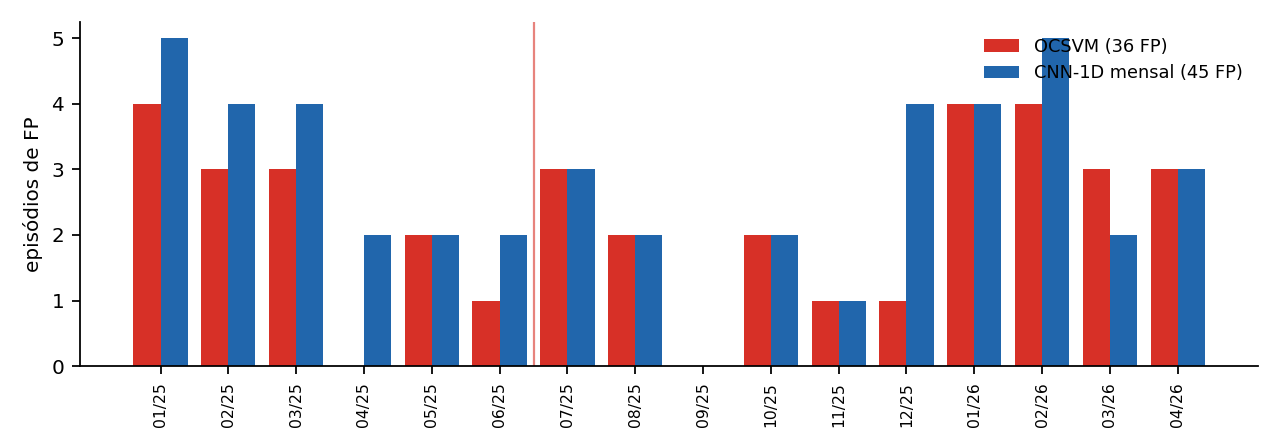
\includegraphics[width=0.85\textwidth]{fp_mensal.png}
\caption{FP por mês nas duas famílias (do relatório OCSVM $\times$ CNN-1D).}
\end{figure}

%=====================================================================
\section{Composição: FP e trips nascem do mesmo jeito}
\label{sec:composicao}
%=====================================================================

Dos 62 episódios da OCSVM desde 01/2025, 61 têm o canal 4 aceso, e 60 deles por \tg{PI_6240319_AL},
\tg{PAL_6240315} ou as duas. O segundo voto vem de um modelo, quase sempre a vibração.

\begin{table}[H]
\centering\small
\caption{OCSVM desde 01/2025: o que acendeu o canal 4 e qual modelo estava aceso, por classe.}
\begin{tabular}{lrrr}
\toprule
 & trips (8) & FP (36) & inconclusivos (18) \\
\midrule
canal 4 por \tg{PI_6240319_AL} e \tg{PAL_6240315} & 3 & 13 & 11 \\
canal 4 só por \tg{PI_6240319_AL} & 4 & 12 & 3 \\
canal 4 só por \tg{PAL_6240315} & 1 & 10 & 3 \\
outra tag ou sem alarme & 0 & 1 & 1 \\
\midrule
modelo aceso: vibração & 6 & 23 & 11 \\
modelo aceso: temperatura & 1 & 4 & 2 \\
modelo aceso: óleo & 1 & 4 & 1 \\
dois modelos & 0 & 5 & 4 \\
\bottomrule
\end{tabular}
\end{table}

As duas tags do canal 4 são alarmes \textbf{recorrentes}: tocam centenas de vezes, e só 7--10\% das ativações ficam
perto de um trip (Tabela~\ref{tab:recorrencia}). O canal 4 fica aceso 45\% do tempo de operação. Na prática, ele é o
``fundo'' sobre o qual a vibração decide: quando a vibração da OCSVM acende (12\% do tempo de operação), há quase
uma chance em duas de o canal 4 já estar aceso.

\begin{table}[H]
\centering\small
\caption{Tags do catálogo mais recorrentes desde 07/2024. ``Perto de trip'': de 48~h antes a 24~h depois.}
\label{tab:recorrencia}
\begin{tabular}{lllll}
\toprule
tag & ativações & perto de trip & \% perto de trip & canal 4 \\
\midrule
PI\_6240319\_AL & 409 & 27 & 7 & sim \\
PAL\_6240315 & 326 & 31 & 10 & sim \\
TC382\_03\_A & 142 & 8 & 6 &  \\
PAL\_6240339 & 136 & 4 & 3 &  \\
PALL\_6240340 & 121 & 4 & 3 &  \\
PDAL\_6240302 & 51 & 7 & 14 & sim \\
T5\_AVG\_A & 50 & 1 & 2 &  \\
TAL\_6240325 & 40 & 2 & 5 &  \\
TAH\_6240305 & 40 & 14 & 35 &  \\
TC382\_05\_A & 38 & 1 & 3 & sim \\
TC382\_01\_A & 35 & 1 & 3 &  \\
TALL\_6240325 & 32 & 2 & 6 &  \\
PAH\_6240319 & 31 & 7 & 23 & sim \\
TC382\_02\_A & 31 & 1 & 3 &  \\
TC382\_04\_A & 30 & 1 & 3 &  \\
TC382\_06\_A & 30 & 1 & 3 &  \\
\bottomrule
\end{tabular}

\end{table}

\begin{figure}[H]
\centering
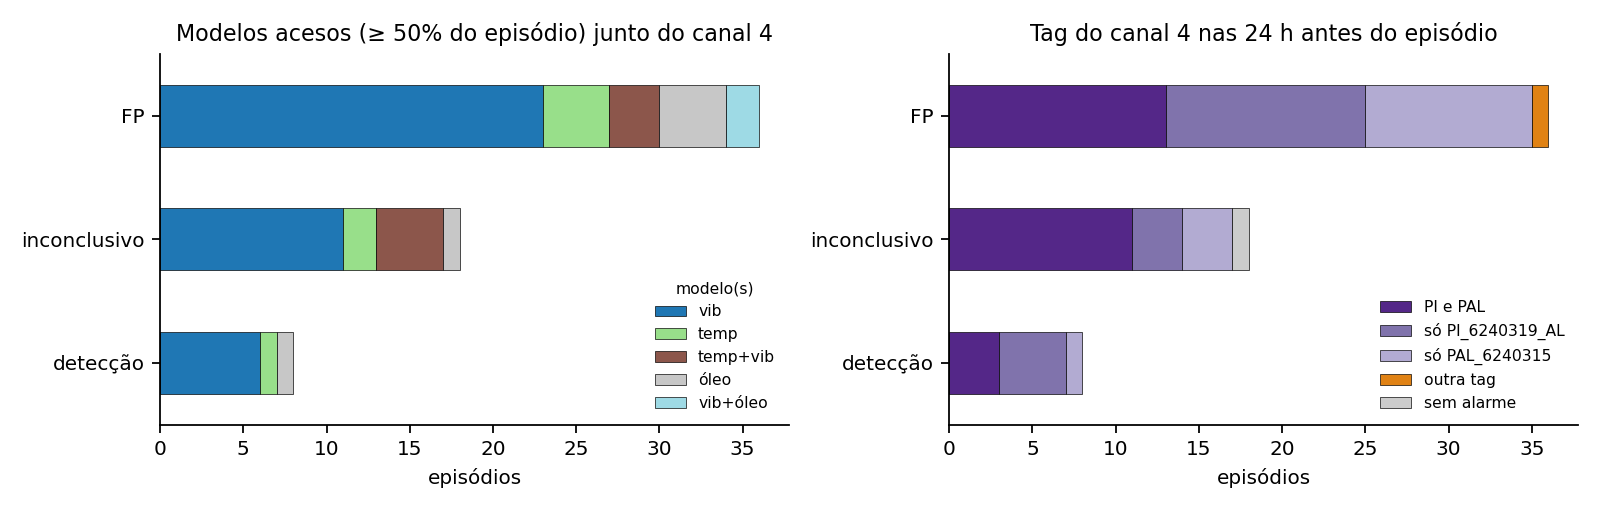
\includegraphics[width=0.9\textwidth]{composicao_episodios.png}
\caption{Composição dos episódios da OCSVM por classe (do relatório OCSVM $\times$ CNN-1D).}
\end{figure}

\textbf{Consequência:} qualquer regra que corte por tag ou por modelo corta trips na mesma proporção que FP.

%=====================================================================
\section{Hipóteses testadas para separar trip de FP}
\label{sec:hipoteses}
%=====================================================================

Todas as hipóteses abaixo foram pré-registradas (critério e expectativa escritos e versionados antes de rodar). O
critério de aceite, quando havia regra, foi: manter os 8 trips, os 3 de fora da amostra, e cortar pelo menos 25\% dos
FP. Escolher parâmetros vendo os mesmos 8 trips infla o resultado, então a escolha foi feita deixando um trip de fora
por vez (LOEO).

\begin{table}[H]
\centering\small
\caption{Hipóteses testadas. AUC = probabilidade de um trip estar mais ``do lado trip'' que um FP (0,5 = acaso).}
\begin{tabular}{l >{\raggedright\arraybackslash}p{6.3cm} >{\raggedright\arraybackslash}p{6.8cm}}
\toprule
teste & hipótese & resultado \\
\midrule
A3 & escolher tags, janela, filtro e refratário do canal 4 & em LOEO cai para 5/8: a escolha atual é seleção \\
B1 & contar o alarme só depois de um silêncio (debounce) & corta no máximo 0,14 FP/mês \\
B2 & janela do canal 4 junto com o filtro de duração & $-32\%$ dentro da amostra vira $-4\%$ fora \\
B3 & alerta ``alto'' só com 2 modelos juntos & rebaixa os 5 trips de 2025; fora, 3/3 em alta (hipótese para dados novos) \\
B5 & o FP antecede um alarme novo & não, abaixo do acaso \\
D2 & CNN-1D de vibração como confirmação & $-6\%$ de FP, mantém 8/8 \\
D3 & score contínuo da OCSVM: magnitude, persistência, carga & não separa (AUC 0,40--0,47) \\
D3b & o mesmo com o CNN-1D mensal & não separa (AUC 0,34--0,40) \\
E2 & alarme ``novo'' (canal 4 aceso há pouco, poucas ativações) & não separa (AUC 0,55 e 0,34) \\
\bottomrule
\end{tabular}
\end{table}

Os testes de score (D3, D3b) têm um resultado que vale ser dito: os FP têm score \emph{maior} e \emph{mais
persistente} que os trips, nas duas famílias. Os modelos não estão errando ``por pouco'' nos FP: eles veem, nesses
momentos, uma anomalia tão forte quanto a dos trips.

\subsection{E2: a novidade do alarme}

A hipótese vinha da gestão de alarmes (ISA-18.2): um alarme crônico perde valor, e o alarme que importa seria o que
aparece depois de dias apagado. Foram medidas duas coisas no momento do alerta: há quanto tempo o canal 4 estava aceso
(N1) e quantas ativações das 5 tags houve nos 7 dias antes (N2). N1 vai na direção esperada (mediana de 3,8~h nos
trips e 14,6~h nos FP), mas é fraco e desaparece fora da amostra. Três trips chegam com o canal 4 aceso há 26 a 74~h.
N2 vai contra a hipótese: os trips acontecem em semanas com \emph{mais} alarme (Figura~\ref{fig:novidade}).

\begin{figure}[H]
\centering
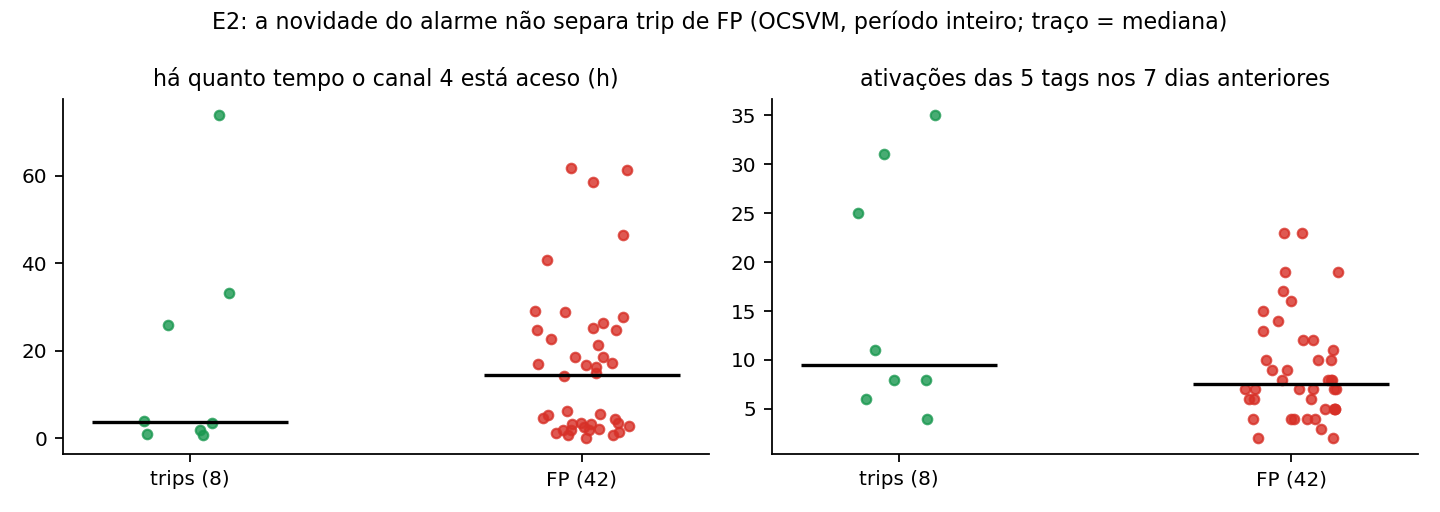
\includegraphics[width=0.9\textwidth]{novidade.png}
\caption{E2: idade do canal 4 aceso e recorrência de alarmes nos 8 trips e nos 42 FP (OCSVM, período inteiro).}
\label{fig:novidade}
\end{figure}

%=====================================================================
\section{Triagem: por que cada FP aconteceu}
\label{sec:causas}
%=====================================================================

Como nenhum sinal separa trip de FP, a pergunta muda: em vez de ``como o trip é diferente?'', ``o que estava
acontecendo em cada FP?'' (E1, \tg{frente_ocsvm/e1_triagem_fp.py}). Para cada episódio foi olhada a janela de 6~h
antes do início até o fim, nos sensores do grupo cujo modelo estava aceso. As causas candidatas são:

\begin{itemize}
  \item \textbf{falha de comunicação:} valor \tg{Comm Fail} ou \tg{Out of Serv} no lugar da medida;
  \item \textbf{sinal interpolado:} metade ou mais da janela em trecho de reta (interpolação do historiador);
  \item \textbf{sensor parado:} leitura constante por 10~min ou mais (a produção já veta 30~min);
  \item \textbf{partida:} o episódio começa até 6~h depois de a máquina voltar a operar;
  \item \textbf{rajada:} 5 ou mais tags de temperatura alarmando em 10~min, nas 24~h em volta;
  \item \textbf{regime pós-27/02/2026:} depois que \tg{PI_6240319_AL} parou de alarmar;
  \item \textbf{alarme crônico:} a tag que acendeu o canal 4 alarmou 10 ou mais vezes em 7 dias.
\end{itemize}

Uma causa só justifica uma regra se \textbf{nenhum trip} a tiver. Os trips entram aqui só como controle.

\begin{figure}[H]
\centering
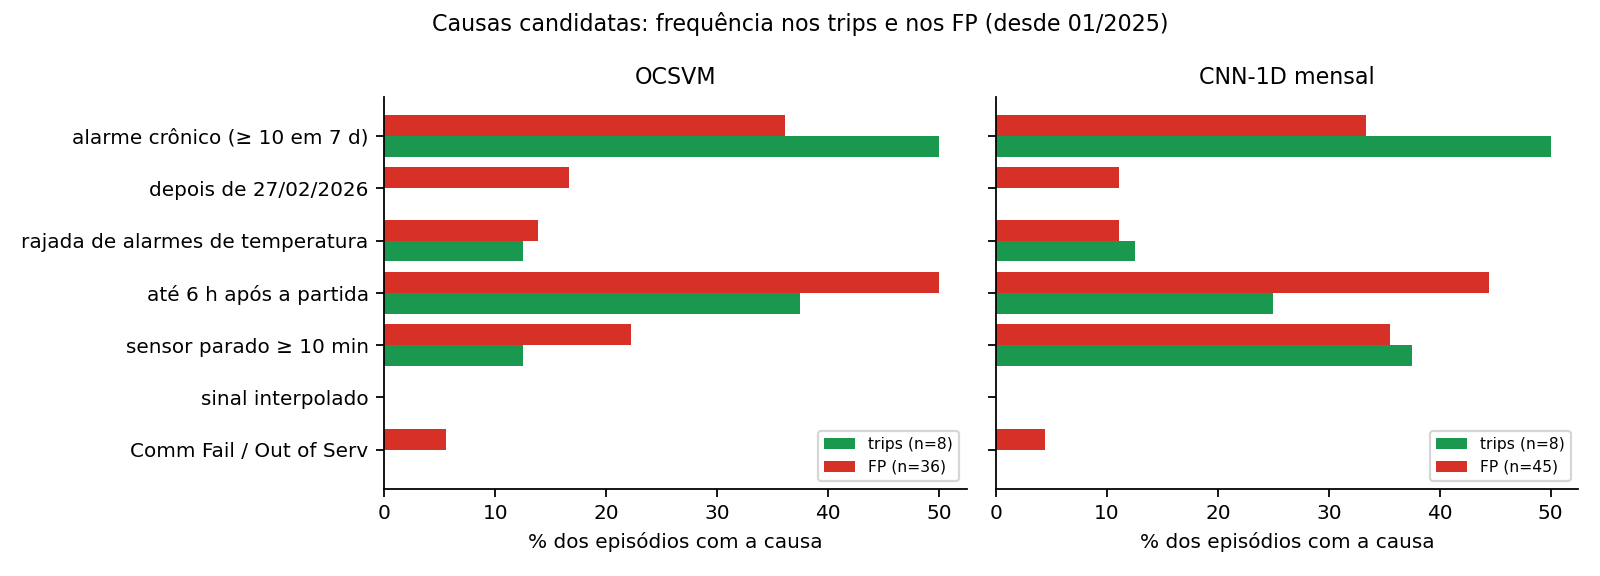
\includegraphics[width=\textwidth]{causas.png}
\caption{Frequência de cada causa candidata nos trips e nos FP, desde 01/2025.}
\label{fig:causas}
\end{figure}

\begin{table}[H]
\centering\small
\caption{Quantos episódios têm cada causa (podem ter mais de uma), desde 01/2025.}
\begin{tabular}{lrrrrl}
\toprule
 & \multicolumn{2}{c}{OCSVM} & \multicolumn{2}{c}{CNN-1D mensal} & \\
causa & trips & FP & trips & FP & serve para regra? \\
\midrule
falha de comunicação & 0 & 2 & 0 & 2 & sim, mas pequena \\
sinal interpolado & 0 & 0 & 0 & 0 & não ocorre \\
sensor parado $\geq$ 10~min & 1 & 8 & 3 & 16 & não \\
até 6~h após a partida & 3 & 18 & 2 & 20 & não do jeito simples \\
rajada de temperatura & 1 & 5 & 1 & 5 & não (T4) \\
depois de 27/02/2026 & 0 & 6 & 0 & 5 & não testável (nenhum trip depois) \\
alarme crônico & 4 & 13 & 4 & 15 & não \\
\bottomrule
\end{tabular}
\end{table}

\subsection{Categoria principal de cada FP}

Para ler os FP como grupos, cada um recebeu uma categoria principal: a primeira, nesta ordem, que se aplica. A ordem
é falha de comunicação, partida ($\leq 2$~h), rajada, série de vibração de 31/01 a 14/02/2026, regime pós-27/02/2026,
alarme crônico e, por último, sem causa identificada.

\begin{table}[H]
\centering\small
\caption{FP por categoria principal, desde 01/2025.}
\begin{tabular}{lrr}
\toprule
categoria & OCSVM (36) & CNN-1D mensal (45) \\
\midrule
partida ($\leq 2$~h após voltar a operar) & 16 & 16 \\
série de vibração 31/01--14/02/2026 & 5 & 6 \\
regime pós-27/02/2026 & 4 & 3 \\
alarme crônico & 4 & 5 \\
falha de comunicação & 2 & 2 \\
rajada de temperatura & 1 & 2 \\
sem causa identificada & 4 & 11 \\
\bottomrule
\end{tabular}
\end{table}

\begin{figure}[H]
\centering
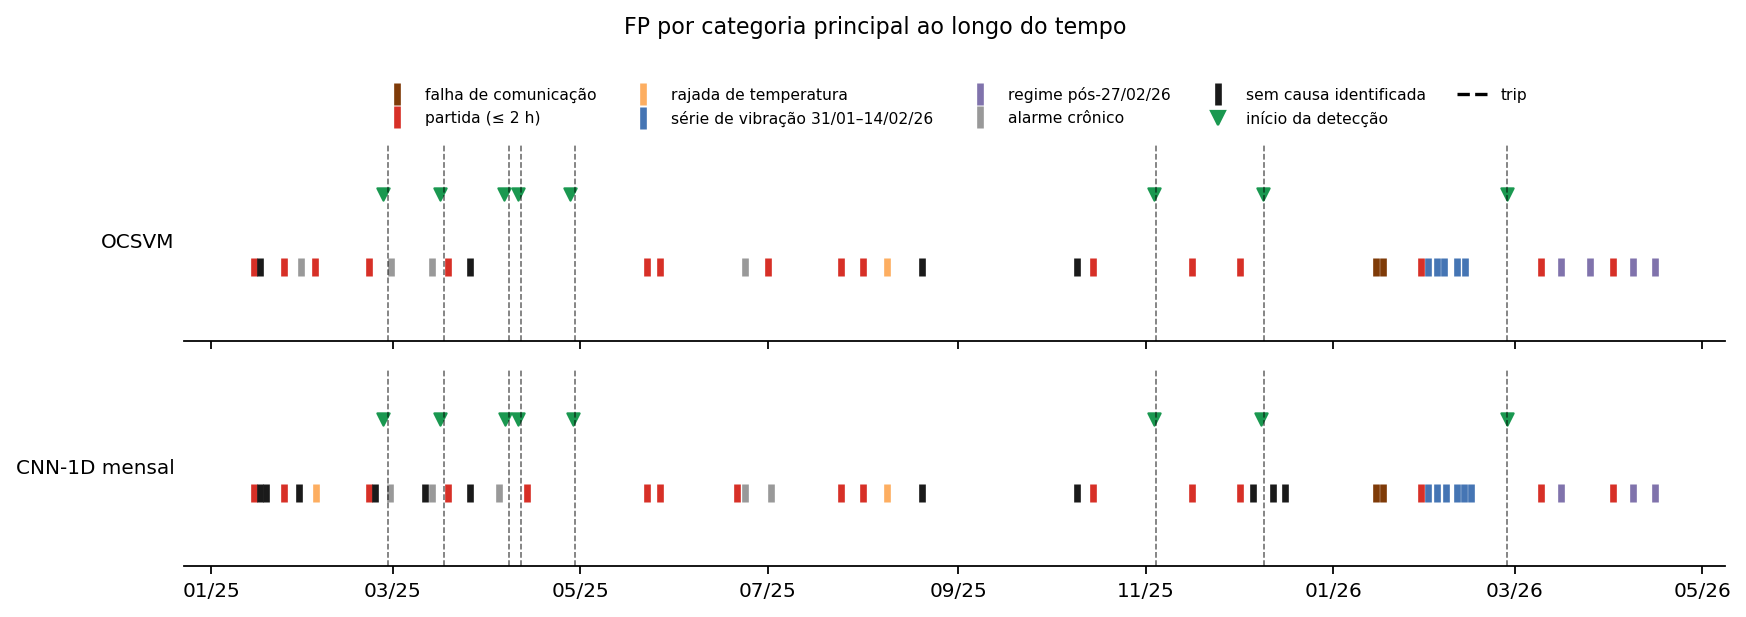
\includegraphics[width=\textwidth]{linha_tempo_fp.png}
\caption{FP ao longo do tempo, coloridos pela categoria principal, com os trips (tracejado) e o início de cada
detecção (triângulo).}
\label{fig:linhatempo}
\end{figure}

\subsection{O grupo maior: logo depois da partida}
\label{sec:partida}

Quinze dos 36 FP da OCSVM (e 15 dos 45 do CNN-1D) começam na \textbf{primeira hora} depois de a máquina voltar ao
estado ``em operação''. Isso acontece mesmo com a produção já descartando 60~min de transitório: o estado ``em
operação'' só começa depois desse intervalo. Ou seja, a máquina ainda está se acomodando quando os modelos voltam a
olhar, e a vibração, sobretudo, sai do padrão do normal de treino.

O problema é que \textbf{três trips também começam ali}: T4 (1,1~h após a partida), T6 (0,6~h) e T7 (0,0~h). Uma
regra que descartasse alertas da primeira hora mataria os três. Esses trips, porém, só acontecem 8 a 20~h depois do
início do episódio. Isso abre uma possibilidade que ainda não foi testada: \textbf{adiar} o alerta nas primeiras
horas após a partida em vez de descartá-lo, e alertar só se a anomalia continuar depois da janela.

\paragraph{Teste do adiamento (E4) -- não funciona.} O adiamento foi pré-registrado e testado
(\tg{frente_ocsvm/e4_adia_partida.py}, commit \tg{f7a2895}): os votos deixam de contar nas primeiras $h$ horas após a
partida, e o alerta só sai se o voto seguir aceso por 45~min depois disso. Com $h = 1$~h, os 8 trips continuam
detectados com antecedência quase igual, mas os FP caem só 5\% (0\% fora da amostra). Com $h \geq 3$~h perde-se o T4.
O motivo é o achado mais útil: \textbf{dos 17 FP de partida, 15 apenas reaparecem} até 8~h depois. A anomalia
pós-partida não é um pico de transitório. É um \emph{regime} de várias horas que os modelos veem como fora do
normal. Para atacá-lo, é preciso mexer no modelo: incluir esse regime no normal de treino, ou usar um limiar próprio
para ele.

\begin{figure}[H]
\centering
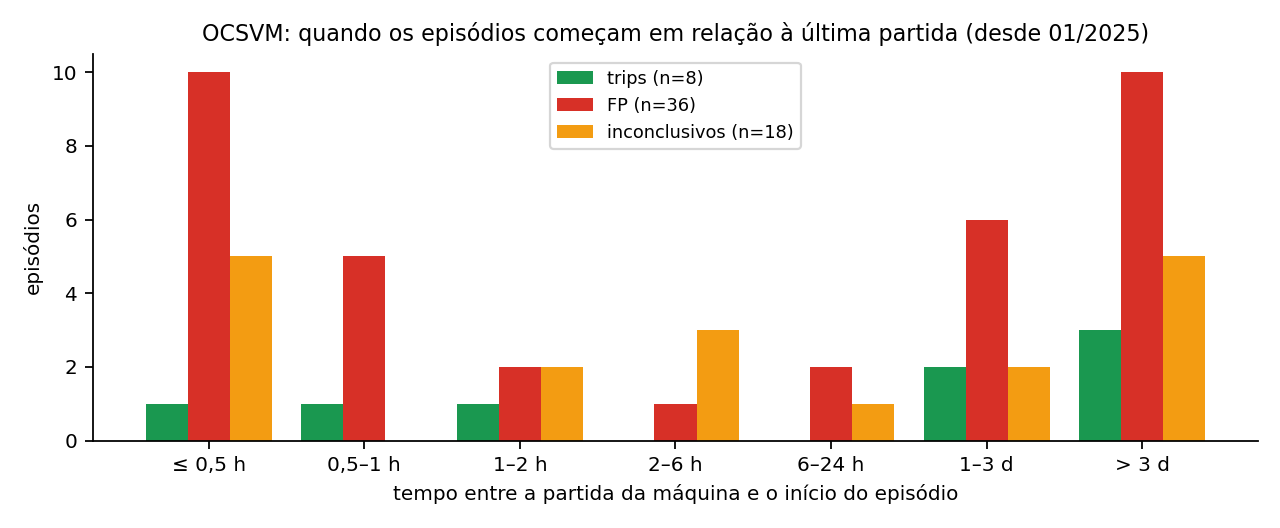
\includegraphics[width=0.9\textwidth]{partida.png}
\caption{Tempo entre a última partida e o início do episódio, por classe (OCSVM, desde 01/2025).}
\label{fig:partida}
\end{figure}

\subsection{Os outros grupos}

\begin{itemize}
  \item \textbf{Série de vibração de 31/01 a 14/02/2026} (5 FP na OCSVM, 6 no CNN-1D). A vibração fica acesa por duas
        semanas, com \tg{PI_6240319_AL} tocando por cima. É provavelmente \emph{um} evento físico, contado como vários
        FP porque o refratário de 48~h libera um alerta novo a cada dois dias (Figura~\ref{fig:serie}). Sem
        registro de manutenção não se sabe se foi um problema real que não levou a trip ou um efeito de
        instrumentação.
  \item \textbf{Regime pós-27/02/2026} (4 e 3 FP; todos os 6 FP desse período têm o canal 4 aceso só por
        \tg{PAL_6240315}). \tg{PI_6240319_AL} parou de alarmar um dia depois do T8, sem registro do motivo. Como não
        há trip depois disso, não dá para saber se o canal 4 ``novo'' ainda serve.
  \item \textbf{Falha de comunicação} (2 FP, 14 e 17/01/2026). É a única causa que nenhum trip tem. Uma regra
        ``ignorar alerta quando o sensor do grupo aceso estiver em falha'' é fisicamente justa, mas corta só 2 FP
        (cerca de $-5\%$).
  \item \textbf{Rajada de temperatura} (1 e 2 FP como causa principal; aparece em 5 FP no total). Vários alarmes de
        temperatura no mesmo segundo, sem mudança no sinal, o que sugere evento de instrumentação. Mas o T4 também
        tem rajada (Figura~\ref{fig:rajadafp}).
  \item \textbf{Sem causa identificada} (4 e 11 FP). Concentram-se em 01--03/2025 e 12/2025. Exigem informação de
        fora dos dados (manutenção, manobra, operação).
\end{itemize}

\begin{figure}[H]
\centering
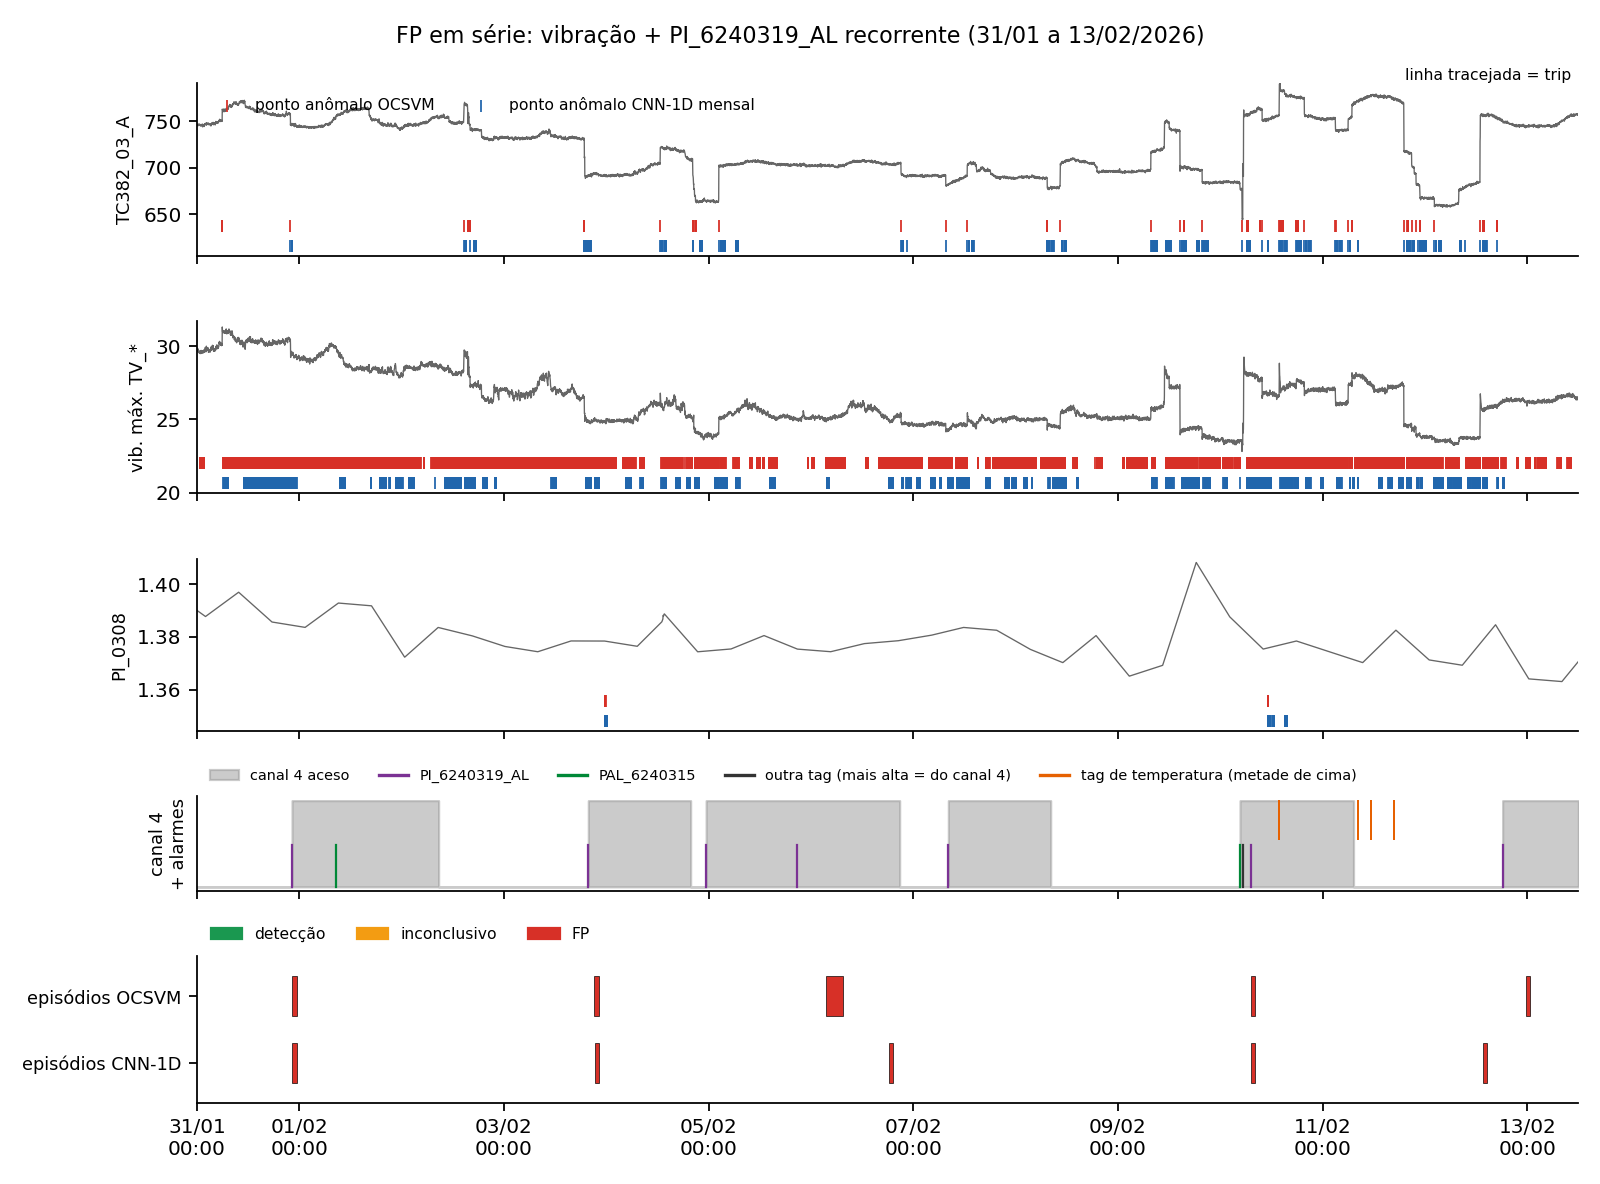
\includegraphics[width=0.92\textwidth]{zoom_fp_chattering.png}
\caption{A série de vibração de 31/01 a 13/02/2026: vibração acesa e \tg{PI_6240319_AL} recorrente geram vários FP
seguidos (do relatório OCSVM $\times$ CNN-1D).}
\label{fig:serie}
\end{figure}

\begin{figure}[H]
\centering
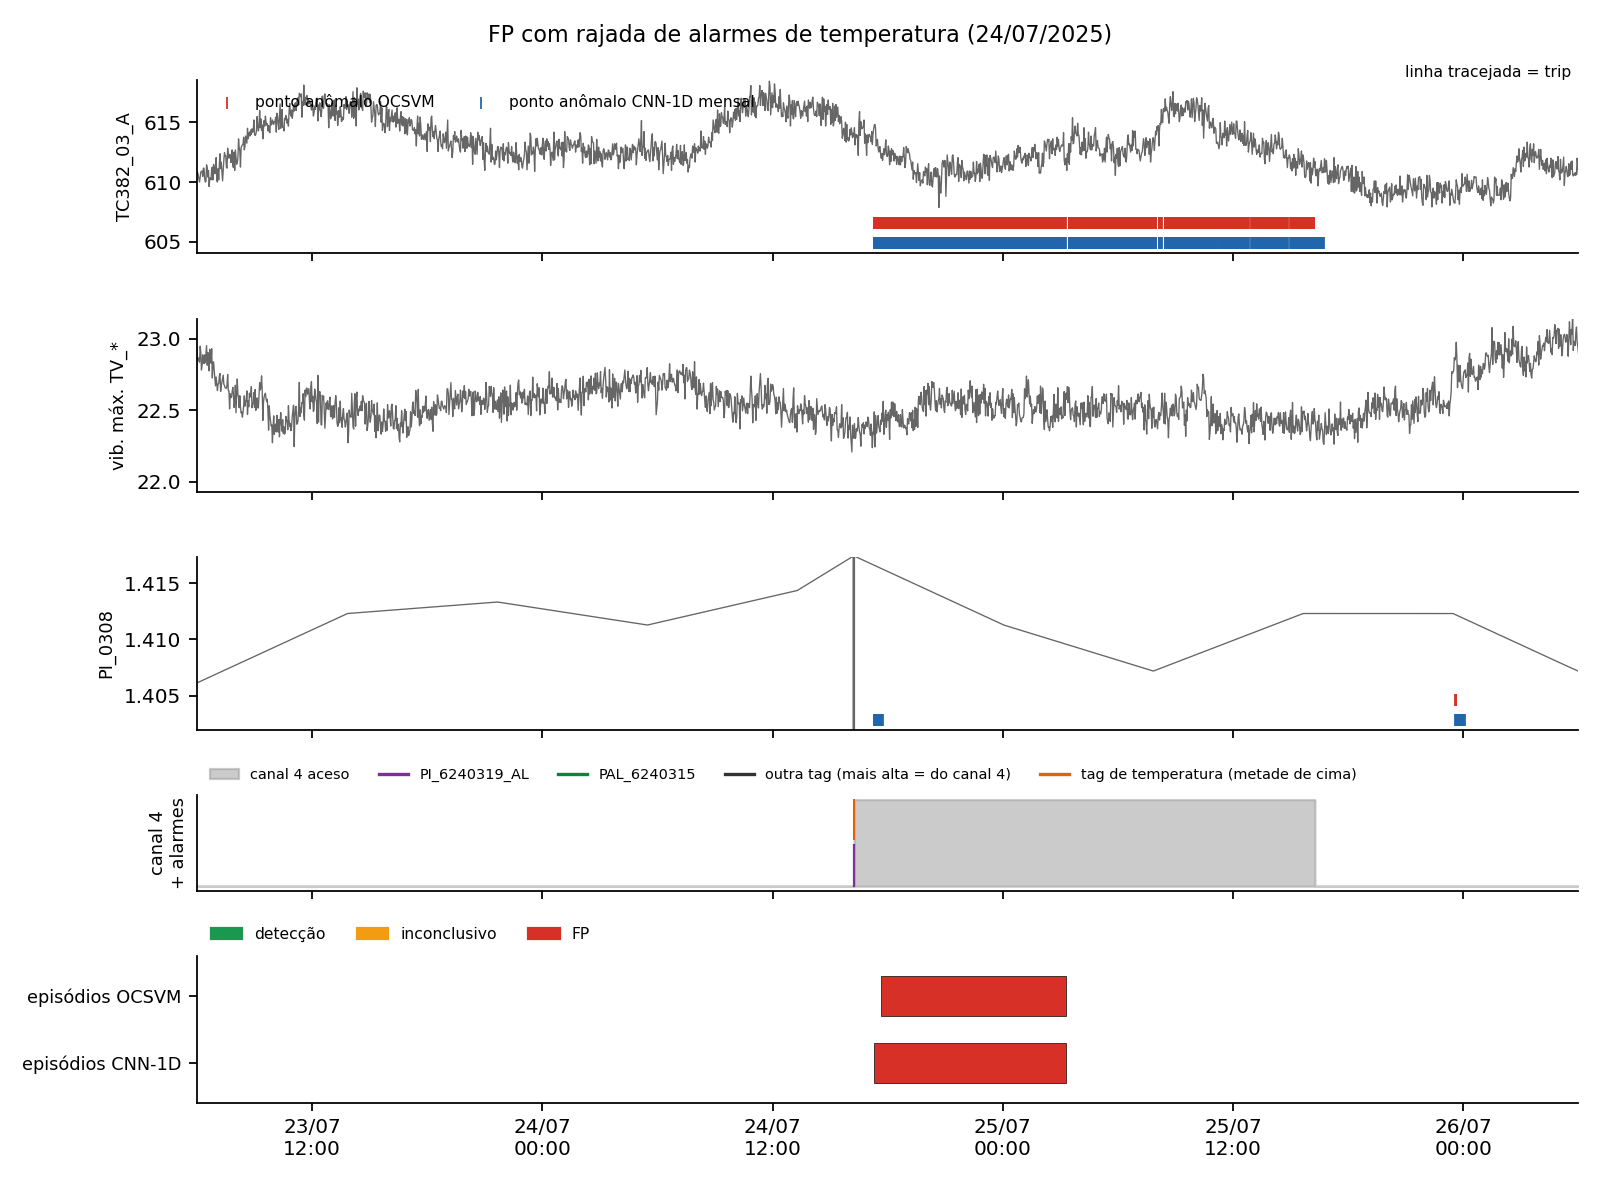
\includegraphics[width=0.92\textwidth]{zoom_fp_rajada.png}
\caption{FP de 24/07/2025 com rajada de alarmes de temperatura no mesmo segundo.}
\label{fig:rajadafp}
\end{figure}

%=====================================================================
\section{A curva de compromisso}
\label{sec:compromisso}
%=====================================================================

Se nada separa trip de FP, a única forma de reduzir FP com os dados atuais é aceitar perder trips. A curva abaixo
(E3, \tg{frente_ocsvm/e3_curva_compromisso.py}) mostra o preço, com dois botões:
\begin{itemize}
  \item \textbf{sensibilidade:} o canal de cada modelo só conta se o score passar $k$ vezes o limiar ($k = 1$ é a
        produção);
  \item \textbf{camada de decisão:} o melhor ponto da grade do A3 para cada número de trips. Foi escolhido olhando os
        trips, então é um teto otimista.
\end{itemize}

\begin{table}[H]
\centering\small
\caption{Pontos da curva (OCSVM de produção, período inteiro 07/2024--04/2026). Fora = desde 01/07/2025, 3 trips.}
\begin{tabular}{lllll}
\toprule
ponto & trips & FP/mês (todo o período) & fora & FP/mês fora \\
\midrule
produção ($k=1$) & 8/8 & 2,885 & 3/3 & 2,877 \\
$k=3$ & 7/8 (perde T2) & 2,335 ($-19\%$) & 3/3 & 2,627 ($-9\%$) \\
$k=4$ a $12$ & 6/8 (T2, T4) & 2,06--2,13 ($-27\%$) & 3/3 & 2,502 ($-13\%$) \\
$k=16$ & 5/8 & 1,854 ($-36\%$) & 3/3 & 2,502 ($-13\%$) \\
A3: só PI + PAL (otimista) & 8/8 & 2,404 ($-17\%$) & 3/3 & 2,251 ($-22\%$) \\
A3: 7 trips (otimista) & 7/8 & 1,923 ($-33\%$) & 3/3 & 2,251 ($-22\%$) \\
\bottomrule
\end{tabular}
\end{table}

\begin{figure}[H]
\centering
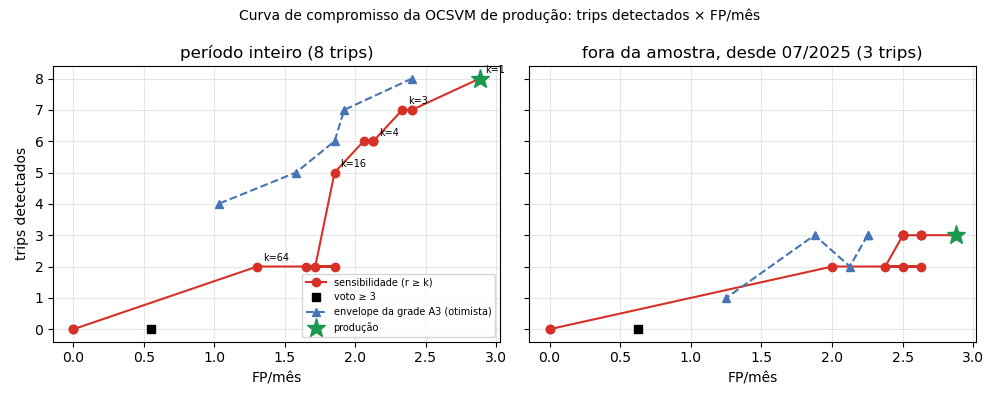
\includegraphics[width=\textwidth]{curva_compromisso.png}
\caption{Trips detectados $\times$ FP/mês, no período inteiro e fora da amostra.}
\label{fig:compromisso}
\end{figure}

\textbf{Não há ponto ``de graça''.} No período inteiro, cada trip a menos economiza cerca de 0,2--0,3 FP/mês. Fora da
amostra, os 3 trips resistem até $k=16$, porque o score deles fica bem acima do limiar. Os FP de fora, porém, também
resistem, e o corte para em $-13\%$. A escolha do ponto é da operação: depende de quanto custa atender um FP comparado
a um trip não previsto.

%=====================================================================
\section{O que falta para explicar o resto}
\label{sec:dados}
%=====================================================================

Os FP que restam não têm explicação nos dados que temos. Cada grupo aponta para uma informação específica:

\begin{table}[H]
\centering\small
\begin{tabular}{>{\raggedright\arraybackslash}p{4.8cm} >{\raggedright\arraybackslash}p{10.4cm}}
\toprule
grupo de FP & dado que o explicaria \\
\midrule
partida & horário e tipo de cada partida (normal, após trip, após manutenção) e o procedimento de aquecimento; o
estado ``em operação'' hoje é inferido do sinal \\
série de vibração 01--02/2026 & ordens de serviço e inspeções da vibração no período \\
regime pós-27/02/2026 & registro de mudança de configuração do \tg{PI_6240319_AL}, e trips depois de 20/04/2026 \\
falha de comunicação e rajadas & eventos do sistema de aquisição (falhas, reinícios, manutenção de instrumentos) \\
sem causa & rótulo das paradas e registro de operação (manobras, testes) \\
todos & trips novos com a pipeline congelada: cada trip novo vale mais que qualquer reanálise dos 8 atuais \\
\bottomrule
\end{tabular}
\end{table}

%=====================================================================
\section{Próximos passos}
%=====================================================================

\begin{enumerate}
  \item \textbf{Tratar o regime pós-partida no modelo.} O adiamento (E4) não funcionou porque a anomalia dura horas.
        O próximo passo é incluir as horas pós-partida no normal de treino, ou dar a elas um limiar próprio. Exige
        retreino no Cica e pré-registro. O risco está nos T4, T6 e T7, que começam na partida.
  \item \textbf{Regra de falha de comunicação: adotada} (E5, \tg{frente_ocsvm/e5_falha_comunicacao.py}). O canal
        do modelo não vota se algum sensor do grupo teve \tg{Comm Fail}/\tg{Out of Serv} nas últimas 6~h. Mantém
        8/8 com as mesmas antecedências, e o FP cai de 42 para 41 (2,885 $\to$ 2,816 por mês). Está na pipeline
        final, que agora também grava a causa provável de cada episódio (``contexto do alerta'': pós-partida,
        repetição em 7 dias, rajada, falha de comunicação, alarme crônico). Esse contexto descreve, mas não separa:
        6 dos 8 trips e 22 dos 41 FP tiveram outro alerta nos 7 dias anteriores.
  \item \textbf{Escolha de ponto da curva} pela operação, se o custo dos FP atuais for alto demais.
  \item \textbf{Pedido de dados} da Seção~\ref{sec:dados}, sobretudo o registro de partidas e de manutenção.
\end{enumerate}

\appendix
\section{Os 36 FP da OCSVM desde 01/2025}

Colunas: início do episódio; modelo aceso; tag que acendeu o canal 4 nas 24~h antes; categoria principal; horas desde
a última partida; ativações das tags do canal 4 em 7 dias; outras causas candidatas presentes.

{\footnotesize\setlength{\tabcolsep}{3pt}
\begin{longtable}{l >{\raggedright\arraybackslash}p{1.4cm} >{\raggedright\arraybackslash}p{2.4cm} >{\raggedright\arraybackslash}p{2.9cm} r r >{\raggedright\arraybackslash}p{3.6cm}}
\toprule
início & modelo & gatilho do canal 4 & categoria & h pós partida & alarm. 7 d & outras causas \\
\midrule
\endhead
14/01/25 17:57 & vib & PI e PAL & partida ($\leq$ 2 h) & 0,6 & 9 &  \\
16/01/25 18:43 & vib & só PI\_6240319\_AL & sem causa identificada & 49,4 & 2 &  \\
24/01/25 12:42 & temp+vib & PI e PAL & partida ($\leq$ 2 h) & 0,4 & 13 & sensor parado $\geq$ 10 min, alarme crônico ($\geq$ 10 em 7 d) \\
30/01/25 03:24 & vib & PI e PAL & alarme crônico & 135,1 & 10 & alarme crônico ($\geq$ 10 em 7 d) \\
03/02/25 16:05 & temp & PI e PAL & partida ($\leq$ 2 h) & 0,0 & 14 & rajada de alarmes de temperatura, alarme crônico ($\geq$ 10 em 7 d) \\
21/02/25 03:27 & vib+óleo & PI e PAL & partida ($\leq$ 2 h) & 0,2 & 6 & sensor parado $\geq$ 10 min \\
28/02/25 08:43 & óleo & PI e PAL & alarme crônico & 14,0 & 12 & sensor parado $\geq$ 10 min, alarme crônico ($\geq$ 10 em 7 d) \\
13/03/25 14:21 & vib & PI e PAL & alarme crônico & 96,7 & 10 & alarme crônico ($\geq$ 10 em 7 d) \\
18/03/25 21:03 & vib & PI e PAL & partida ($\leq$ 2 h) & 0,1 & 19 & alarme crônico ($\geq$ 10 em 7 d) \\
26/03/25 02:31 & temp & só PAL\_6240315 & sem causa identificada & 46,8 & 1 &  \\
22/05/25 17:57 & vib & PI e PAL & partida ($\leq$ 2 h) & 1,0 & 16 & alarme crônico ($\geq$ 10 em 7 d) \\
26/05/25 22:33 & temp & só PI\_6240319\_AL & partida ($\leq$ 2 h) & 0,0 & 17 & rajada de alarmes de temperatura, alarme crônico ($\geq$ 10 em 7 d) \\
23/06/25 14:04 & óleo & só PI\_6240319\_AL & alarme crônico & 62,2 & 14 & sensor parado $\geq$ 10 min, alarme crônico ($\geq$ 10 em 7 d) \\
01/07/25 01:32 & vib & PI e PAL & partida ($\leq$ 2 h) & 0,0 & 19 & alarme crônico ($\geq$ 10 em 7 d) \\
24/07/25 17:39 & temp & só PI\_6240319\_AL & partida ($\leq$ 2 h) & 0,4 & 2 & rajada de alarmes de temperatura \\
31/07/25 23:48 & vib & PI e PAL & partida ($\leq$ 2 h) & 0,9 & 9 &  \\
08/08/25 15:34 & óleo & só PI\_6240319\_AL & rajada de temperatura & 184,7 & 4 & sensor parado $\geq$ 10 min, rajada de alarmes de temperatura \\
20/08/25 00:45 & vib & só PI\_6240319\_AL & sem causa identificada & 26,4 & 4 &  \\
09/10/25 11:35 & vib & só PI\_6240319\_AL & sem causa identificada & 23,3 & 2 &  \\
14/10/25 21:15 & vib & PI e PAL & partida ($\leq$ 2 h) & 1,4 & 10 & alarme crônico ($\geq$ 10 em 7 d) \\
15/11/25 22:00 & vib & só PAL\_6240315 & partida ($\leq$ 2 h) & 0,5 & 11 & alarme crônico ($\geq$ 10 em 7 d) \\
01/12/25 14:27 & vib+óleo & só PAL\_6240315 & partida ($\leq$ 2 h) & 0,0 & 11 & sensor parado $\geq$ 10 min, alarme crônico ($\geq$ 10 em 7 d) \\
14/01/26 18:57 & vib & só PAL\_6240315 & falha de comunicação & 0,6 & 5 & Comm Fail / Out of Serv, rajada de alarmes de temperatura \\
17/01/26 01:00 & óleo & só PI\_6240319\_AL & falha de comunicação & 54,7 & 2 & Comm Fail / Out of Serv, sensor parado $\geq$ 10 min \\
29/01/26 13:17 & temp+vib & PI e PAL & partida ($\leq$ 2 h) & 1,2 & 7 & sensor parado $\geq$ 10 min \\
31/01/26 22:18 & vib & só PI\_6240319\_AL & série de vibração 31/01–14/02/26 & 58,2 & 4 &  \\
03/02/26 21:02 & vib & só PI\_6240319\_AL & série de vibração 31/01–14/02/26 & 129,0 & 4 &  \\
06/02/26 03:28 & vib & só PI\_6240319\_AL & série de vibração 31/01–14/02/26 & 183,4 & 4 &  \\
10/02/26 07:14 & vib & só PAL\_6240315 & série de vibração 31/01–14/02/26 & 283,2 & 2 &  \\
12/02/26 23:46 & vib & só PI\_6240319\_AL & série de vibração 31/01–14/02/26 & 347,7 & 3 &  \\
09/03/26 12:07 & vib & só PAL\_6240315 & partida ($\leq$ 2 h) & 0,7 & 7 & depois de 27/02/2026 \\
16/03/26 02:50 & vib & só PAL\_6240315 & regime pós-27/02/26 & 159,4 & 5 & depois de 27/02/2026 \\
25/03/26 09:33 & vib & só PAL\_6240315 & regime pós-27/02/26 & 382,1 & 2 & depois de 27/02/2026 \\
01/04/26 23:34 & vib & só PAL\_6240315 & partida ($\leq$ 2 h) & 0,5 & 4 & depois de 27/02/2026 \\
08/04/26 09:44 & vib & só PAL\_6240315 & regime pós-27/02/26 & 2,9 & 8 & depois de 27/02/2026 \\
15/04/26 14:43 & temp+vib & outra tag & regime pós-27/02/26 & 175,9 & 2 & depois de 27/02/2026 \\
\bottomrule
\end{longtable}

}

\noindent Arquivos:
\begin{itemize}
  \item \tg{relatorio_falsos_positivos/gera_figuras_fp.py}: figuras, tabela do apêndice e \tg{numeros.json};
  \item \tg{frente_ocsvm/e1_triagem_fp.py}: triagem por causa (E1);
  \item \tg{frente_ocsvm/e2_novidade_alarme.py}: novidade do alarme (E2);
  \item \tg{frente_ocsvm/e3_curva_compromisso.py}: curva de compromisso (E3);
  \item \tg{DIARIO_DE_BORDO.md}: registro.
\end{itemize}

\end{document}
